\documentclass[10pt,twocolumn,letterpaper]{article}
%\usepackage[latin1]{inputenc}

%\usepackage{url}
%\usepackage{booktabs}

\usepackage{cvpr}
\usepackage{times}
\usepackage{epsfig}
\usepackage{graphicx}
\usepackage{amsmath}
\usepackage{amssymb}
\usepackage{amsmath}
\usepackage{amsfonts}
\usepackage{subfigure}
\usepackage{nonfloat}
\usepackage{url}
\graphicspath{{imgs/}}

\usepackage{xspace}
%\newcommand*{\eg}{e.g.\@\xspace}
%\newcommand*{\ie}{i.e.\@\xspace}
\newcommand*{\ea}{et al.\@\xspace}
%\renewcommand{\arraystretch}{1.5}

\cvprfinalcopy % *** Uncomment this line for the final submission

\def\cvprPaperID{****} % *** Enter the CVPR Paper ID here
\def\httilde{\mbox{\tt\raisebox{-.5ex}{\symbol{126}}}}

\newcommand{\prob}{Pr}
\newcommand{\rgbdimage}{\mathbf{I}}
\newcommand{\imregion}{\mathcal{R}}
\newcommand{\occ}{o}
\newcommand{\basisshape}{B}
\newcommand{\pcloud}{\mathcal{P}}
\newcommand{\point}{\mathbf{p}}
\newcommand{\normal}{\mathbf{n}}
\newcommand{\ray}{\mathbf{R}}
\newcommand{\degree}{^{\circ}}

\title{Predicting Voxel Occupancy From a Single RGBD Image}

\author{Michael Firman, Gabriel Brostow, Simon Julier \ea}

\begin{document}


\maketitle

\begin{abstract}
	Gaining a representation of the geometry of a scene is an essential task for many applications including robotic navigation, scene re-lighting and object manipulation. 
	Most existing works to recover the scene geometry rely on combining multiple views of the scene captured from many different directions or use of \emph{a priori} information about the expected semantic make-up of the scene.

	We present a method to predict whether or not each voxel in a scene is occupied given just a single RGBD image.
	We argue that objects of dissimilar semantic classes often share similar shapes; this allows for a limited dataset of CAD objects to model the shape of a wide range of objects and hence estimate the hidden geometry of arbitrary scenes.

	Our method comprises of three main components:
	1) For each pixel in an RGBD image, we compute local and regional features and use these to predict the thickness of the object at that point, using a Random Forest trained on multiple CAD models.
	2) To extend occluded surfaces
	3) Finally we combine and regularise the thickness predictions and occluded surface continuations to form a full probablistic distribution of occupancy for each voxel in the scene.
\end{abstract}


\section{Introduction}
Given a single image of a scene, humans can usually get a good overview of the scene and what the geometry is, even in the many areas which are not directly observable. 
We are able to do this using a manner of different tools at our disposal. 
We can use symmetry, hypothesising that unobserved regions match the parts we can see under a transform.
In many occasions we exploit semantic knowledge: by recognising specific objects and relating them to objects in our memory, we form an idea of their shape.
In many cases, however, we use a more generic, higher level knowledge about shape in order to hypothesise the missing regions.


\paragraph{Application areas}
It can be very useful for a computer system to know the geometry of hidden areas of a scene, for reasons such as:

\begin{itemize}
\item \textbf{Robotics} --- Helping a robot to plan a path around objects given only a single view of a scene, e.g. from a doorway. Also to help a robot plan grasping position on objects it can only see partial views of.
\item \textbf{Scene relighting} --- Enabling realistic-looking shadows to be cast from a light moved to a new position in the image.
\item \textbf{Object repositioning} --- Interactive repositioning of objects in the scene. Knowing the voxel occupancy allows a constraint to be placed on where objects can be moved to. (\eg Zheng \ea, Interactive images)
\item \textbf{Multi-view reconstruction} --- An intial estimate for voxel occuapncy can be used as a prior during online multi-view reconstruction algorithms. This prior prediction would be overwritten with observed data as more footage is captured.
\end{itemize}

\paragraph{Aim of the system and overview}
Given a single RGBD image, the aim of our system is to predict whether each voxel in the scene is occupied or not - in effect, we want to predict the voxelised occupancy grid of KinectFusion \cite{izadi-uist-2011}, but having been given only a single view of the scene instead of multiple views.

We [plan to] achieve this by matching each region from the input image to a similar region of an object in a training database.
The thickness of the object is then used.
Because we care about voxel occupancy, and not semantic understanding, we are free to use training objects which differ in scale and semantic labelling from the objects being modelled in the scene. 
This is key to our approach --- we are not reasoning about semantics of objects, but instead about object shape.
In effect we are hypothesising that any two objects that have a similar shape from one angle are likely to share similarities in shape in the unobserved regions of the scene.

Of course the problem is ill-posed; we therefore can only hope to make a reasonable guess of the occupancy and we rely on the predictability and repeatability of the world.

%In addition, our output can act as a prior for algorithms such as registration.

% \subsubsection{What is our hypothesis?}

% What is our overall hypotheses --- that the shape we can see from one angle is enough information to make a sensible prediction about the parts of the scene which are occluded?

% We aren't making assumptions about class, unlike \eg shotton (people) or room modelling.

\subsubsection{Motivation for using a voxelised world}

Voxels can be expensive compared to point clouds and meshes. 
However they are a very natural representation of our world, and have been shown to work well for reconstruction \eg KinFu and other voxel carving papers. 
With tools such as OpenVDB\footnote{\url{www.openvdb.org}}, voxelised representations of objects can be stored and manipulated efficiently.

% \begin{quote}
% Voxel occupancy is one approach for reconstructing the 3-dimensional shape of an object from multiple views. In voxel occupancy, the task is to produce a binary labeling of a set of voxels, that determines which voxels are filled and which are empty.

% \cite{snow-cvpr-2000}
% \end{quote}

% In addition, our world remains at the same resolution, while computers are becoming larger and more powerful. 
% People have make work-arounds for efficiently using voxels in very large ares, \eg Kintinuous.


% \begin{figure}
%   \centering 
%   \subfigure[Example input image]{%
%       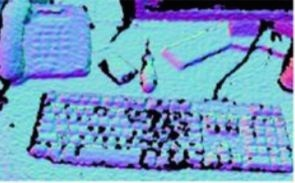
\includegraphics[width=0.4\columnwidth]{kinfu1.jpg}}
%       \hfill
%   \subfigure[Ground truth output]{%
%       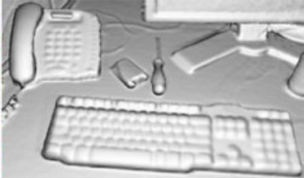
\includegraphics[width=0.4\columnwidth]{kinfu2.jpg}} \\
%   \caption{Given a single RGBD image (\eg (a)), the aim is to predict the full, occupied volume of the scene (e.g. (b)).}
% \end{figure}

\paragraph{Motivation from other areas}
Shape sharing...

\subsubsection{Contributions}
\begin{itemize}
\item A novel feature representation for a point which captures both local and region-level shape, while respecting occlusions.
\item A regularisation system for combining depth and surface predictions
\end{itemize}

\subsubsection{Problem statement}

Setting out the problem mathematically, introducing some notation etc.

% What exactly do we mean by voxel occupancy?

% What is the scope of the work? 

% %%%%%%%%%%%%%%%%%%%%%%%%%%%%%%%%%%%%%%%%%%%%%%%%%%%%%%%%%%%%%%%%%%%%%%%%%%%%%%%%
\section{Related work}
% %%%%%%%%%%%%%%%%%%%%%%%%%%%%%%%%%%%%%%%%%%%%%%%%%%%%%%%%%%%%%%%%%%%%%%%%%%%%%%%%

% \paragraph{Axes of variation of related works}
% Using local information (\eg smoothing) $\leftrightarrow$ using global information (\eg patching from other images)

% Parametric models (Gaussian smoothing, CRFs) $\leftrightarrow$ non-parametric (patch-based)

% Care about semantic matching $\leftrightarrow$ Don't care about semantics


\paragraph{Nearest neighbours}
\cite{shen-tog-2012} use an assembly of parts from a CAD database to complete the unseen parts of a model given an RGBD image. 
While they demonstrate good results they assume they have semantic-specific models of the objects in the dataset.
Kim \ea \cite{kim-iccv-2013} use a CRF model over a voxel representation of a scene to simultaneously predict occupancy, visibility and semantical labelling of voxels from an RGBD image. 
For training, they use manually labelled top-down views of the scene. 
Their prediction of occupancy, however, is really just a Gaussian model. 
Final labellings found from graph cuts over the CRF. 
They make the observation that the observed values from a Kinect sensor can be very bad, and may need cleaning up.
%Silberman \ea \cite{silberman-eccv-2014} complete holes in partial KinectFusion meshes of indoor scenes.

Fouhey \ea \cite{fouhey-iccv-2013} use the NYU dataset of RGBD images to learn how to predict the normal orientations for each pixel of an input RGB image. 
In our case we are tackling a similar problem at a higher level --- we take RGBD as input, and aim to predict the full geometry of the scene.

\cite{guo-iccv-2013} use a single RGBD image to estimate the location and extent of the \emph{support surfaces} (\eg tabletops) in the scene. They do this by processing and analsing the geometry, before finally fitting shapes to the hypothesised support regions. They provide user-annotated 3D reconstructions of the full 3D space of the NYU dataset images, which could become useful for our work.


\paragraph{Mesh and image completion}
In the graphics community, there is a lot of work looking at the completion of missing and occluded parts of 3D meshes and 2D images. 
For example, \cite{podolak-esgp-2005} fill holes in a mesh by enforcing watertightness across an octree structure, while \cite{schnabel-eurographics-2009} complete meshes by using primitives extracted from the areas of the scan without missing detail. 
A good overview of such mesh completion algorithms are given in \cite{ju-cst-2009}.

\cite{silberman-eccv-2014} complete meshes from partial KinFU reconstructions, \eg behind items of furniture.
They use this for augmeted realist situations, \eg allowing balls to bounce off floor in unseen areas.
They detect planes in the voxelised representation of the scene, and complete their contours in 2D using a novel CRF method.

Image completion, such as \cite{hays-siggraph-2007, criminisi-cvpr-2003}, typically has the aim of getting a good visually plausible output irrespective of the accuracy compared to ground truth. 
The results can be very impressive. 
\cite{hays-siggraph-2007} look up possible completion regions in a large database of similar images, while \cite{criminisi-cvpr-2003} inpaint by selecting and combining multiple plausible patches from other regions of the input image.

Depth images are a more complex beast than meshes and 2D images, and RGBD datasets on the order of millions of images do not yet exist, so we need to take a different approach.

\paragraph{Super-resolution}
Similar to mesh completion is super-resolution, \eg \cite{macaodha-eccv-2012}. 
This, like our problem, is ill-posed and relies on the repeatability and predictability of the world in order to find suitable matches.
A seminal paper in this field is \cite{freeman-ijcv-2000}, patches from generic training images are used in super-resolution for coarse-grained images. They use Bayesian belief propagation to find the maximum posterior probability over a Markov network defined over the image.

\cite{chang-tor-2007} complete a robot's map of an environment using parts of the already observed world to  `patch in' missing areas of the current map.

\paragraph{Symmetry}
Law and Aliaga \cite{law-cviu-2010} use symmetry to complete partial views. 
They are limited to only completing partial views; they rely on all objects being symmetrical; and they need user input.
Similarly, \cite{thrun-iccv-2005} and \cite{kroemer-humanoids-2012} use symmetry to complete models from a single depth view. 
They both demonstrate results on isolated objects, but not on more complex or cluttered scenes. 
The constraint of requiring axes of symmetry to both be present and accurately detected is a large limiting factor with these approaches.

\paragraph{Indoor room semantic prediction}
These works in general try to understand the semantic layout of a scene, \ie given an image infer what objects are in the scene and what their poses are.
\cite{nan-acm-2012, minkim-siggraphasia-2012}
This could be seen as finding one-to-many correspondences between models in a database and points in the scene.
In our work, by not restricting ourselves to trying to find semantic correspondences, we are able to model the shape of a far greater range of test scenes without making any assumptions about their semantic makeup.

\paragraph{Indoor room occupied space prediction}
\cite{hedau-cvpr-2012} seek to recover the free space in 2D images. They label ~500 images with box annotations, and aim to recover the bounding box layout of the scene in order to recover the free space.

In the vision community, most of the work is based around estimating the spatial layout of rooms from images.
For example \cite{bao-wacv-2014} use multiple images, before SfM and segmentation of the images. 
They then generate hypotheses of the layout. 
The hypotheses are chosen by evaluating their geometric cost, which is manually defined. 
They cite a lot of papers which do scene reasoning from a single image, but they argue that the problem is ill-posed (which it is). 

Using a single image, many people fit bounding boxes and try to estimate the layout using high-level info about gravity, typical scene arrangements etc. 
For example \cite{choi-cvpr-2013}.

\cite{lee-nips-2010} are another paper using a single image to estimate the layout of a room. 
Similarly, \cite{zhang-iccv-2013} infer the clutter and layout and support and segmentation and labelling from an RGBD image (using the NYU dataset).

\cite{hedau-cvpr-2012} seek to recover the free space in 2D images. 
They label ~500 images with box annotations, and aim to recover the bounding box layout of the scene in order to recover the free space. 
A big work in this area is that by \cite{gupta-cvpr-2011}, who estimate voxel occupation before fitting boxes.

Satkin \ea \cite{satkin-bmvc-2012} use 3D models to do scene understanding from a single image, and they demonstrate results on room scenes such as bedrooms and living rooms. 
A key interest for me is that they first propose hypotheses, before rendering them with OpenGL.
This then feeds into a hypothesis scorer which says if their ideas are any good. 
They form their proposals in an expensive way: they moving the cad model along the (x, y) scene axes, and render the model in every location, and in each of 4 rotation configurations!

\paragraph{6DOF object pose estimation}
Our work is closely related to the problem of estimating the 6DOF pose of a known database of objects in cluttered scenes, such as \cite{hinterstoisser-accv-2012, drost-3dimpvt-2012, rusu-iros-2010}. 
These work in many different ways; \cite{drost-3dimpvt-2012} aggregate pairwise features in a hash table to find the pose estimation --- they assume just one database model, which is assumed to be in the scene. \cite{rusu-iros-2010} first segment the scene, before looking up each segment in their training dataset.
All the methods nonetheless share the training step of rendering a 3D object from multiple angles.

All these methods so far assume that the item in the scene has the exact same geometry of the training instances.
\cite{cocias-cgvcv-2013} take an alternative approach, where they have a single primitive object for each class, which they fit to the scene and allow to deform to account for inter-class variation.
\cite{prisacariu-iccv-2011} present a more developed version of this idea, where the latent axes of variation of the shape of the object being fitted are allowed to deform during the pose estimation. 
These latent axes are found using Gaussian processes.

\paragraph{Robotics and path planning}
Voxels or 2D occupancy grids are often used in robotics for path planning, and for maintaining a map of the environment. 
These are typically deterministic approaches, \eg \cite{jetchev-icra-2010}. Sometimes a state model is used to model the states of voxels being occupied, unoccupied or unknown --- the voxel states are then updated as more information is gathered from sensors \cite{toussaint-techreport-2007}.

\cite{stentz-icra-1994} introduced D*, an algorithm similar to A* but for path planing in partially unknown environments. 
The world is in boxes, with arrows pointing to the direction which should be taken.
More recently, \cite{plagemann-iros-2008} used Gaussian processes to fill in missing data in terrain models of environments, effectively treating terrain mapping as a regression problem.

\paragraph{General motivation}
One key motivation is Shape Sharing \cite{kim-eccv-2012}, where silhouettes of objects are used to segment other objects from different classes.
 \cite{nan-acm-2012}.

Big issue with ground truth. Most papers don't have proper ground truth and therefore can only really do qualitative results, \eg \cite{all the papers...}.

\paragraph{Scene relighting}
\cite{ikeda-acpr-2013} perform scene relighting from a single RGBD image, but cannot recover shadows cast by objects in the scene.
On the other hand, \cite{xiao-cvpr-2014} use the RGBD information to automatically \textit{remove} hard and soft shadows from a single image.

\paragraph{Training for scene completion}
Long history of using training scenes to try to complete and upsample.

\paragraph{To add to related work:}
\begin{itemize}
\item Box world --- predicting object locations and extents (and hence unseen completion) through bounding boxes. 
The problem with this is it gives incredibly coarse occupation information.
\item Teaching 3D Geometry to Deformable Part Models
\end{itemize}


% %%%%%%%%%%%%%%%%%%%%%%%%%%%%%%%%%%%%%%%%%%%%%%%%%%%%%%%%%%%%%%%%%%%%%%%%%%%%%%%%
\section{Approach}
% %%%%%%%%%%%%%%%%%%%%%%%%%%%%%%%%%%%%%%%%%%%%%%%%%%%%%%%%%%%%%%%%%%%%%%%%%%%%%%%%

Our approach is somewhat inspired by patch-based methods used for superresolution or similar of depth images. 

% Overview of the method --- Figure \ref{fig:pipeline}.


% General motivation for method. Do not want to rely on having exact matches in training set. 
% Instead, want to find a collection of good matches in the training set which, when combined, will give a sensible prediction of the voxel occupancy.
% We take a RANSAC-style approach to finding basis shapes: first we \emph{propose} a set of candidate shapes which roughly match the scene, before we next \emph{re-weight} these candidates according to how well they match the scene geometry. 


%%%%%%%%%%%%%%%%%%%%%%%%%%%%%%%%%%%%%%%%%%%%%%%%%%%%%%%%%%%%%%%%%%%%%%%%%%%%%%%%%
\section{Thickness prediction}
%%%%%%%%%%%%%%%%%%%%%%%%%%%%%%%%%%%%%%%%%%%%%%%%%%%%%%%%%%%%%%%%%%%%%%%%%%%%%%%%%

The aim of our thickness prediction function is to map a point $\point$ in the image to a scalar thickness $t$.


%%%%%%%%%%%%%%%%%%%%%%%%%%%%%%%%%%%%%%%%%%%%%%%%%%%%%%%%%%%%%%%%%%%%%%%%%%%%%%%%%
\subsection{Edges in depth images}
Describe here:
\begin{itemize}
\item Types of edges (depth, colour, occluding etc)
\item Our method for depth edges
\item motivation - why do we care about occlusions?
\end{itemize}

We reason that discontinuities in depth images can be assigned a direction: one side of each edge is the occluder, the other is the occludee. 
We can compute the gradient of the depth edges using PCA on the edge pixels in image space.
We ensure that the final gradient at each edge pixel points in the direction of the occluded side.

We can then use the occlusion information in our feature computations --- see for example figure \ref{fig:occluded_region}.


\begin{figure}
    \centering 
    \subfigure[]{%
        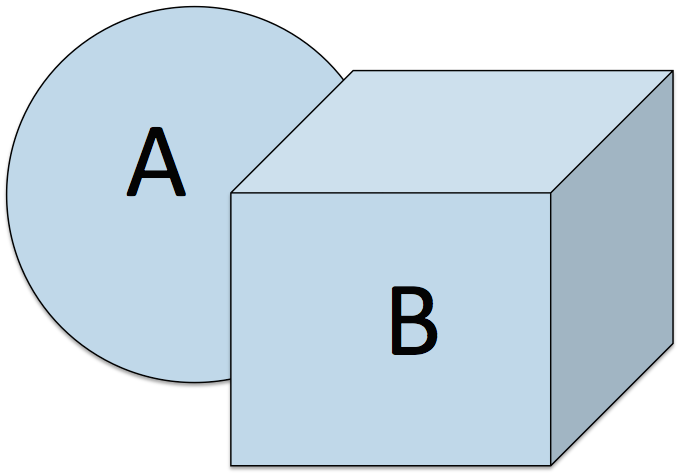
\includegraphics[width=0.45\columnwidth]{occlusion_a}}
        \hfill
    \subfigure[]{%
        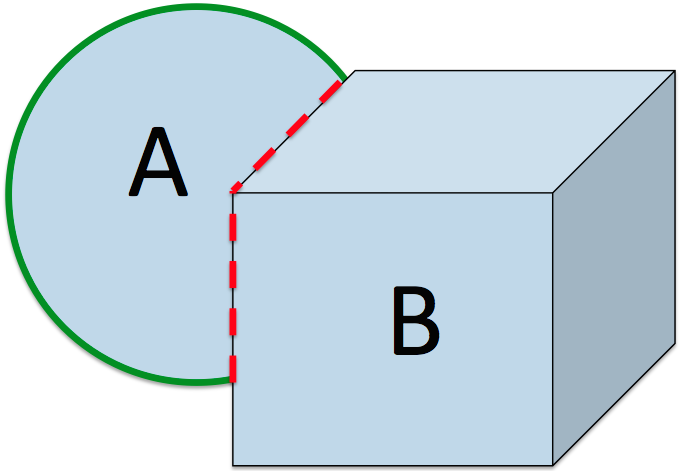
\includegraphics[width=0.45\columnwidth]{occlusion_b}} \\
    \caption{Where edges occur as a result of occlusion boundaries, the direction of the edge is important. The edge bounding region A can be divided into an \emph{occluding} portion (solid green) and an \emph{occluded} portion (dashed red).
    We can make a reasonable assumption that region A may extend behind object B past the occluded edge --- however, region A cannot continue sideways beyond its occluding edge.}
    \label{fig:occluded_region}
\end{figure}



%%%%%%%%%%%%%%%%%%%%%%%%%%%%%%%%%%%%%%%%%%%%%%%%%%%%%%%%%%%%%%%%%%%%%%%%%%%%%%%%%
\subsection{Features}
Our method is to use local and regional featues extracted from the image around $\point$ to predict the thickness of the object at that point.
At each pixel on the dpeth image we compute an angle $\theta$, which represents the direction of the gradient of the depth in the image plane.
Each of the features are computed with respect to the local reference frame defined by $\theta$.
This has the effect of making our features invariant to rotations of objects in the camera plane --- computing our features at the same point on an object which has undergone an in-camera-plane rotation should give the same feature.

%We avoid using region-level features

We use two novel features, which we describe in detail here. See also figure \ref{fig:features}.
%The first, the cobweb feature, captures 


\newcommand{\subwidth}{0.32\columnwidth}
\begin{figure*}
    \centering 
    \subfigure[$\theta$ at each point]{%
        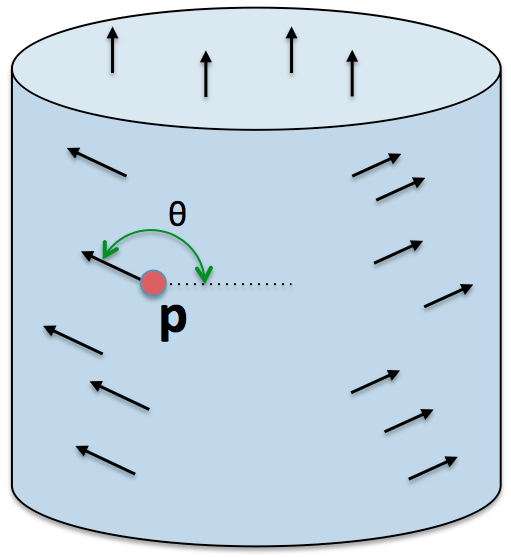
\includegraphics[width=\subwidth]{01_angles}}
        \hfill
    \subfigure[Spider feature]{%
        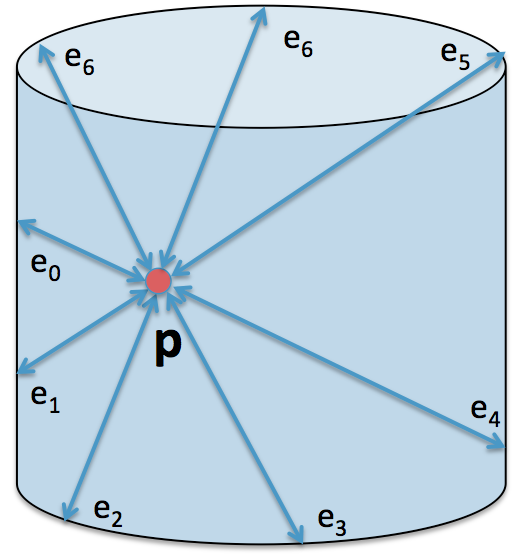
\includegraphics[width=\subwidth]{02_spider}}
        \hfill
    \subfigure[Rotation invariance]{%
        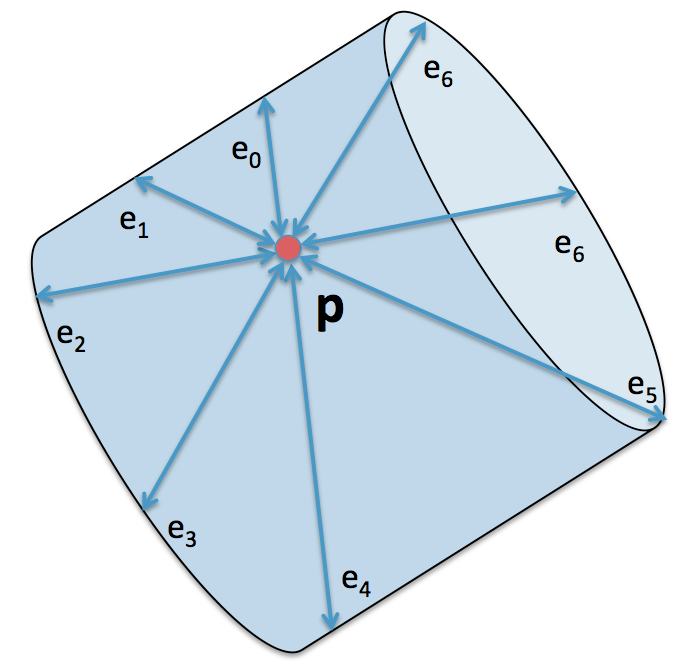
\includegraphics[width=0.4\columnwidth]{03_spider_rot}}
        \hfill
    \subfigure[Occluded spider]{%
        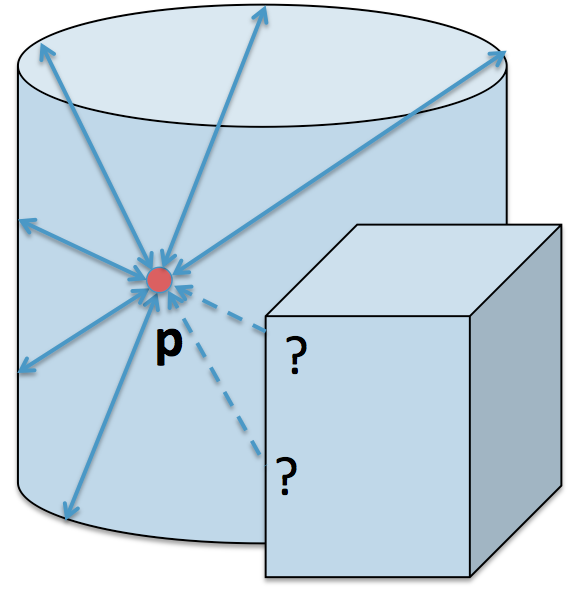
\includegraphics[width=\subwidth]{04_spider_occ}}
        \hfill
    \subfigure[Cobweb feature]{%
        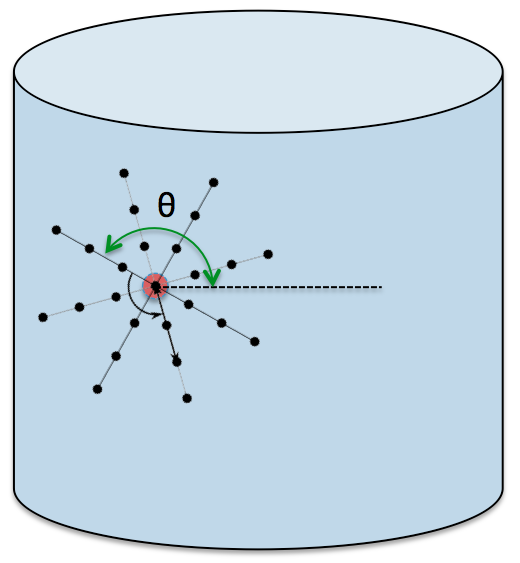
\includegraphics[width=\subwidth]{05_cobweb}}
        \hfill
    \caption{
    (a) Each point on a depth image has an angle $\theta$ associated, which represents the direction of gradient of the depth. 
    (b) The spider features measure the distance between $\point$ and the edge points $e_{1, \cdots, 7}$.
    (c) Because the spider features are computed relative to $\theta$, the resultant feature vector is invariant to object rotations in the camera plane.
    (d) Where the spider line emitted from $\point$ first hits an occluded edge, the true extent is unknown --- this case is denoted as \texttt{?} in this figure.
    (e) The cobweb feature measures the difference in depth between $\point$ and a set of points in the near vicinity of $\point$, arranged in a cobweb shape.
    The cobweb feature is also computed relative to $\theta$.}%
    \label{fig:features}
\end{figure*}


\subsubsection{Cobweb feature}
The cobweb feature captures the surface shape in the immediate vicinity of $\point$. 
It captures very similar data to a patch of the depth image; however, an image patch maintains a constant resolution across the selected region, while the cobweb feature becomes more coarse the further from $\point$ it is.
%This property helps to reflect the 
\begin{align}
f(i, j, \psi, t) &= \rgbdimage_{ij} - \rgbdimage_{ab} \\
a &= \lfloor i + tm\sin(\theta_{ij}+\psi)\rceil \\
b &= \lfloor j + tm\cos(\theta_{ij}+\psi)\rceil \\
m &= \frac{df}{\rgbdimage_{ij}},
\end{align}
where $f$ is the focal length of the camera and $d$ is a fixed constant in real-world coordinates. For our experiements we set $d=0.02m$ and we compute the cobweb feature for $\psi = [0\degree, 45\degree, \ldots, 315\degree]$, and $t = [1, 2, 3]$. 
The final cobweb feature is therefore 24-dimensional.

% Dealing with depth discontinuities?




\subsubsection{Spider features}
The spider feature captures the size and shape of the region in which $\point$ resides. 
Rather than explicitly computing region-level features, however, which may suffer from poor segmentations (and the problem with occlusion), we compute these features capturing the region's shape at the point level. 
We first compute an edge map for the image.
We again consider the set of angles $\phi$. Starting from $\point$, we cast a Bresenham line along the depth image until it hits an edge. 
We denote the point at which the edge was hit as $\point_{e}$.

For each line cast, we store 
a) the geodesic distance between $\point$ and $\point_{e}$ along the depth surface, and 
b) the 3D distance between $\point$ and $\point_{e}$ along the direction of the normal at $\point$. (In practice, we take the point 95\% of the way between $\point$ and $\point_{e}$ in image space, as this helps to prevent problems with poor quality edge data).

The spider feature is therefore 16-dimensional.

We explicitly handle occlusion in the spider features. Where the spider feature first hits an occluded edge rather than an occluding edge, the true size of the object in that dimension is unknown (see figure \ref{fig:occluded_spider}).
We explicitly encode this unknown value --- in practice with \texttt{NaN} --- and the Random Forest can then make a sensible decision about what to do with it.

% \begin{figure}
%     \centering% 
%     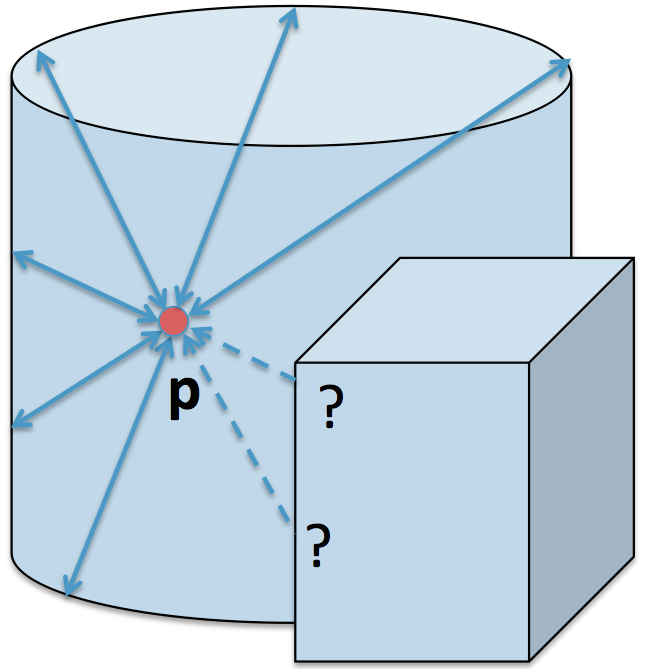
\includegraphics[width=0.7\columnwidth]{occlusion_spider.png}% 
%     \figcaption{The spider feature extends lines from $\point$ to the first occluding edge found along the path. Internal edges (e.g. those found in RGB space) are ignored. Where the line first hits an occluded edge, the true extent is unknown --- this case is denoted as \texttt{?} in this figure.}% 
%     \label{fig:occluded_spider}% 
% \end{figure}




%\subsubsection{}

%%%%%%%%%%%%%%%%%%%%%%%%%%%%%%%%%%%%%%%%%%%%%%%%%%%%%%%%%%%%%%%%%%%%%%%%%%%%%%%%%
\subsection{Learning}

We train a Random Forest using a total of 1,000,000 training examples extracted from 1,600 CAD models, each rendered from 42 different angles.


%%%%%%%%%%%%%%%%%%%%%%%%%%%%%%%%%%%%%%%%%%%%%%%%%%%%%%%%%%%%%%%%%%%%%%%%%%%%%%%%
\section{Datasets used}
%%%%%%%%%%%%%%%%%%%%%%%%%%%%%%%%%%%%%%%%%%%%%%%%%%%%%%%%%%%%%%%%%%%%%%%%%%%%%%%%


%%%%%%%%%%%%%%%%%%%%%%%%%%%%%%%%%%%%%%%%%%%%%%%%%%%%%%%%%%%%%%%%%%%%%%%%%%%%%%%%
\section{Experiments}
%%%%%%%%%%%%%%%%%%%%%%%%%%%%%%%%%%%%%%%%%%%%%%%%%%%%%%%%%%%%%%%%%%%%%%%%%%%%%%%%


\begin{figure}
    \centering% 
    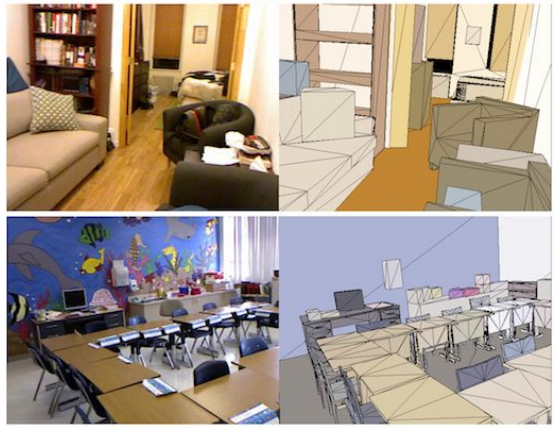
\includegraphics[width=1.0\columnwidth]{guo.png}% 
    \figcaption{Representation of objects in the NYU dataset, provided from \cite{guo-iccv-2013}.
    Not a perfect representation but perhaps reasonable to some extents.}% 
    \label{fig:guo_labels}% 
\end{figure}



\subsection{Database of CAD models}
Use the database from Fisher \ea \cite{fisher-siggraphasia-2012}.
1600 CAD models, each depth-rendered from 42 viewing angles using OpenGL.

\subsubsection{Potential test datasets}
\begin{itemize}
\item Create our own KinFu dataset
\item Kaparthy \ea --- would probably have to re-render their meshes.
Also don't have the TSDF etc. Lots of problems
\item NYU dataset --- classic dataset. Potential ground truth labels from \cite{guo-iccv-2013} (figure \ref{fig:guo_labels}) or \cite{kim-iccv-2013}.
\item \cite{fisher-siggraphasia-2012}, use their synthetic scenes (great for a first pass!)
\end{itemize}

\begin{figure}
    \centering% 
    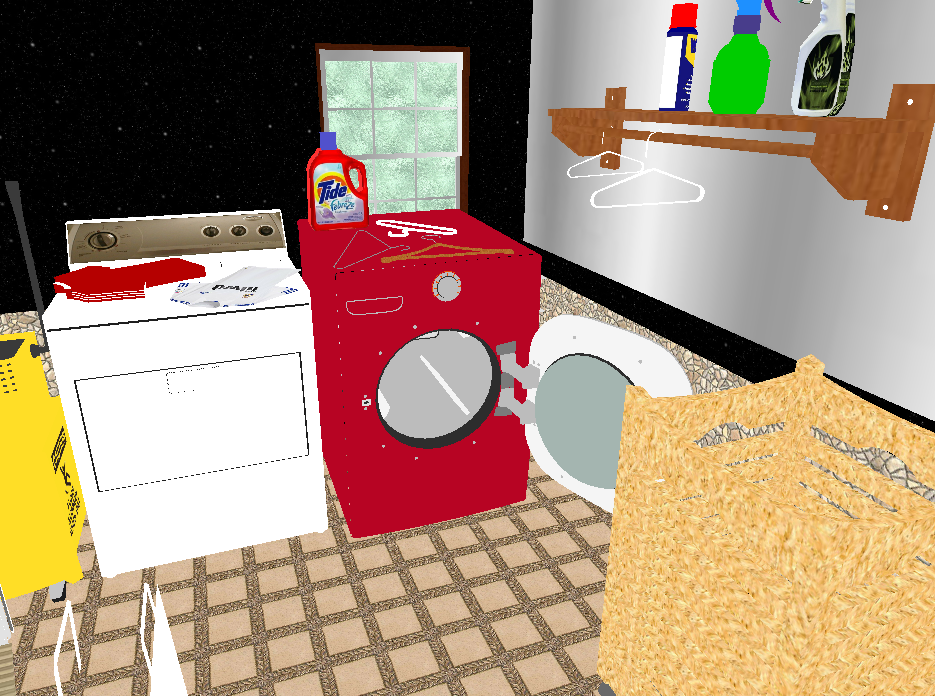
\includegraphics[width=1.0\columnwidth]{synth_scene.png}% 
    \figcaption{One of the user-created synthetic scenes from \cite{fisher-siggraphasia-2012}.}% 
    \label{fig:fisher_scene}% 
\end{figure}

% \section{Acknowledgements}
% Peter Gehler
% Oisin
% Prism group
% Malcolm


%\bibliographystyle{plain}
%\bibliographystyle{apalike}
%\bibliography{bibtex/strings.bib,bibtex/main.bib,bibtex/crossrefs.bib}


{\small
\bibliographystyle{apalike}
\bibliography{bibtex/strings.bib,bibtex/main.bib,bibtex/crossrefs.bib}
}


\end{document}